% -*- latex -*-
% sprawozadanie-szkielet.tex
% LabSK
% ato 2010-2022

\author{Weronika Skiba}                 
\title{Instrukcja podłączenia zasobów Labsk w systemie Android} 

% Grafika w sprawozdaniu wyłącznie w formacie wektorowym (pdf, svg)
% Poza wyjątkowymi sytuacjami nie są akceptowane pliki rastrowe gif png itp.

\frenchspacing                          % Bez spacji na końcu zdania.
%\graphicspath{ {c1} }

\documentclass[a4paper,11pt]{article}

\usepackage[T1]{polski}
\usepackage[utf8]{inputenc}                     % Kodowanie pliku
\usepackage{graphicx}

\hoffset=-3.0cm                         % Mniejszy lewy margines
\textwidth=18cm                         % szerzej
\evensidemargin=0pt

\voffset=-3cm                           % Mniejszy górny margines
\textheight=27cm                        % szerzej wzdłuż
 
\setlength{\parindent}{0pt}             % Paragraf od początku linii
\setlength{\parskip}{\medskipamount}    % Odstęp pomiędzy paragrafami
\raggedbottom                           % bez rozciągania strony

% Dodatkowe komendy
\newcommand\BS{\char`\\}                % \BS == back-slash
\newcommand\TY{\raise.17ex\hbox{$\scriptstyle\mathtt{\sim}$}}   % \TY == większa tylda w \tt

\begin{document}
\maketitle
\begin{center}
\vspace{6 cm}

\includegraphics[scale=1]{logo-pw.jpg} 
\end{center}
\newpage
%\thispagestyle{empty}                  % bez numeracji stron
\section{Pobranie aplikacji}
W serwisie służącym do pobierania aplikacji na urządzenia mobilne (np. Play Store) wyszukujemy aplikację ZeroTier One i pobieramy ją na nasze urządzenie.
\vspace{0.5cm}
\begin{center}
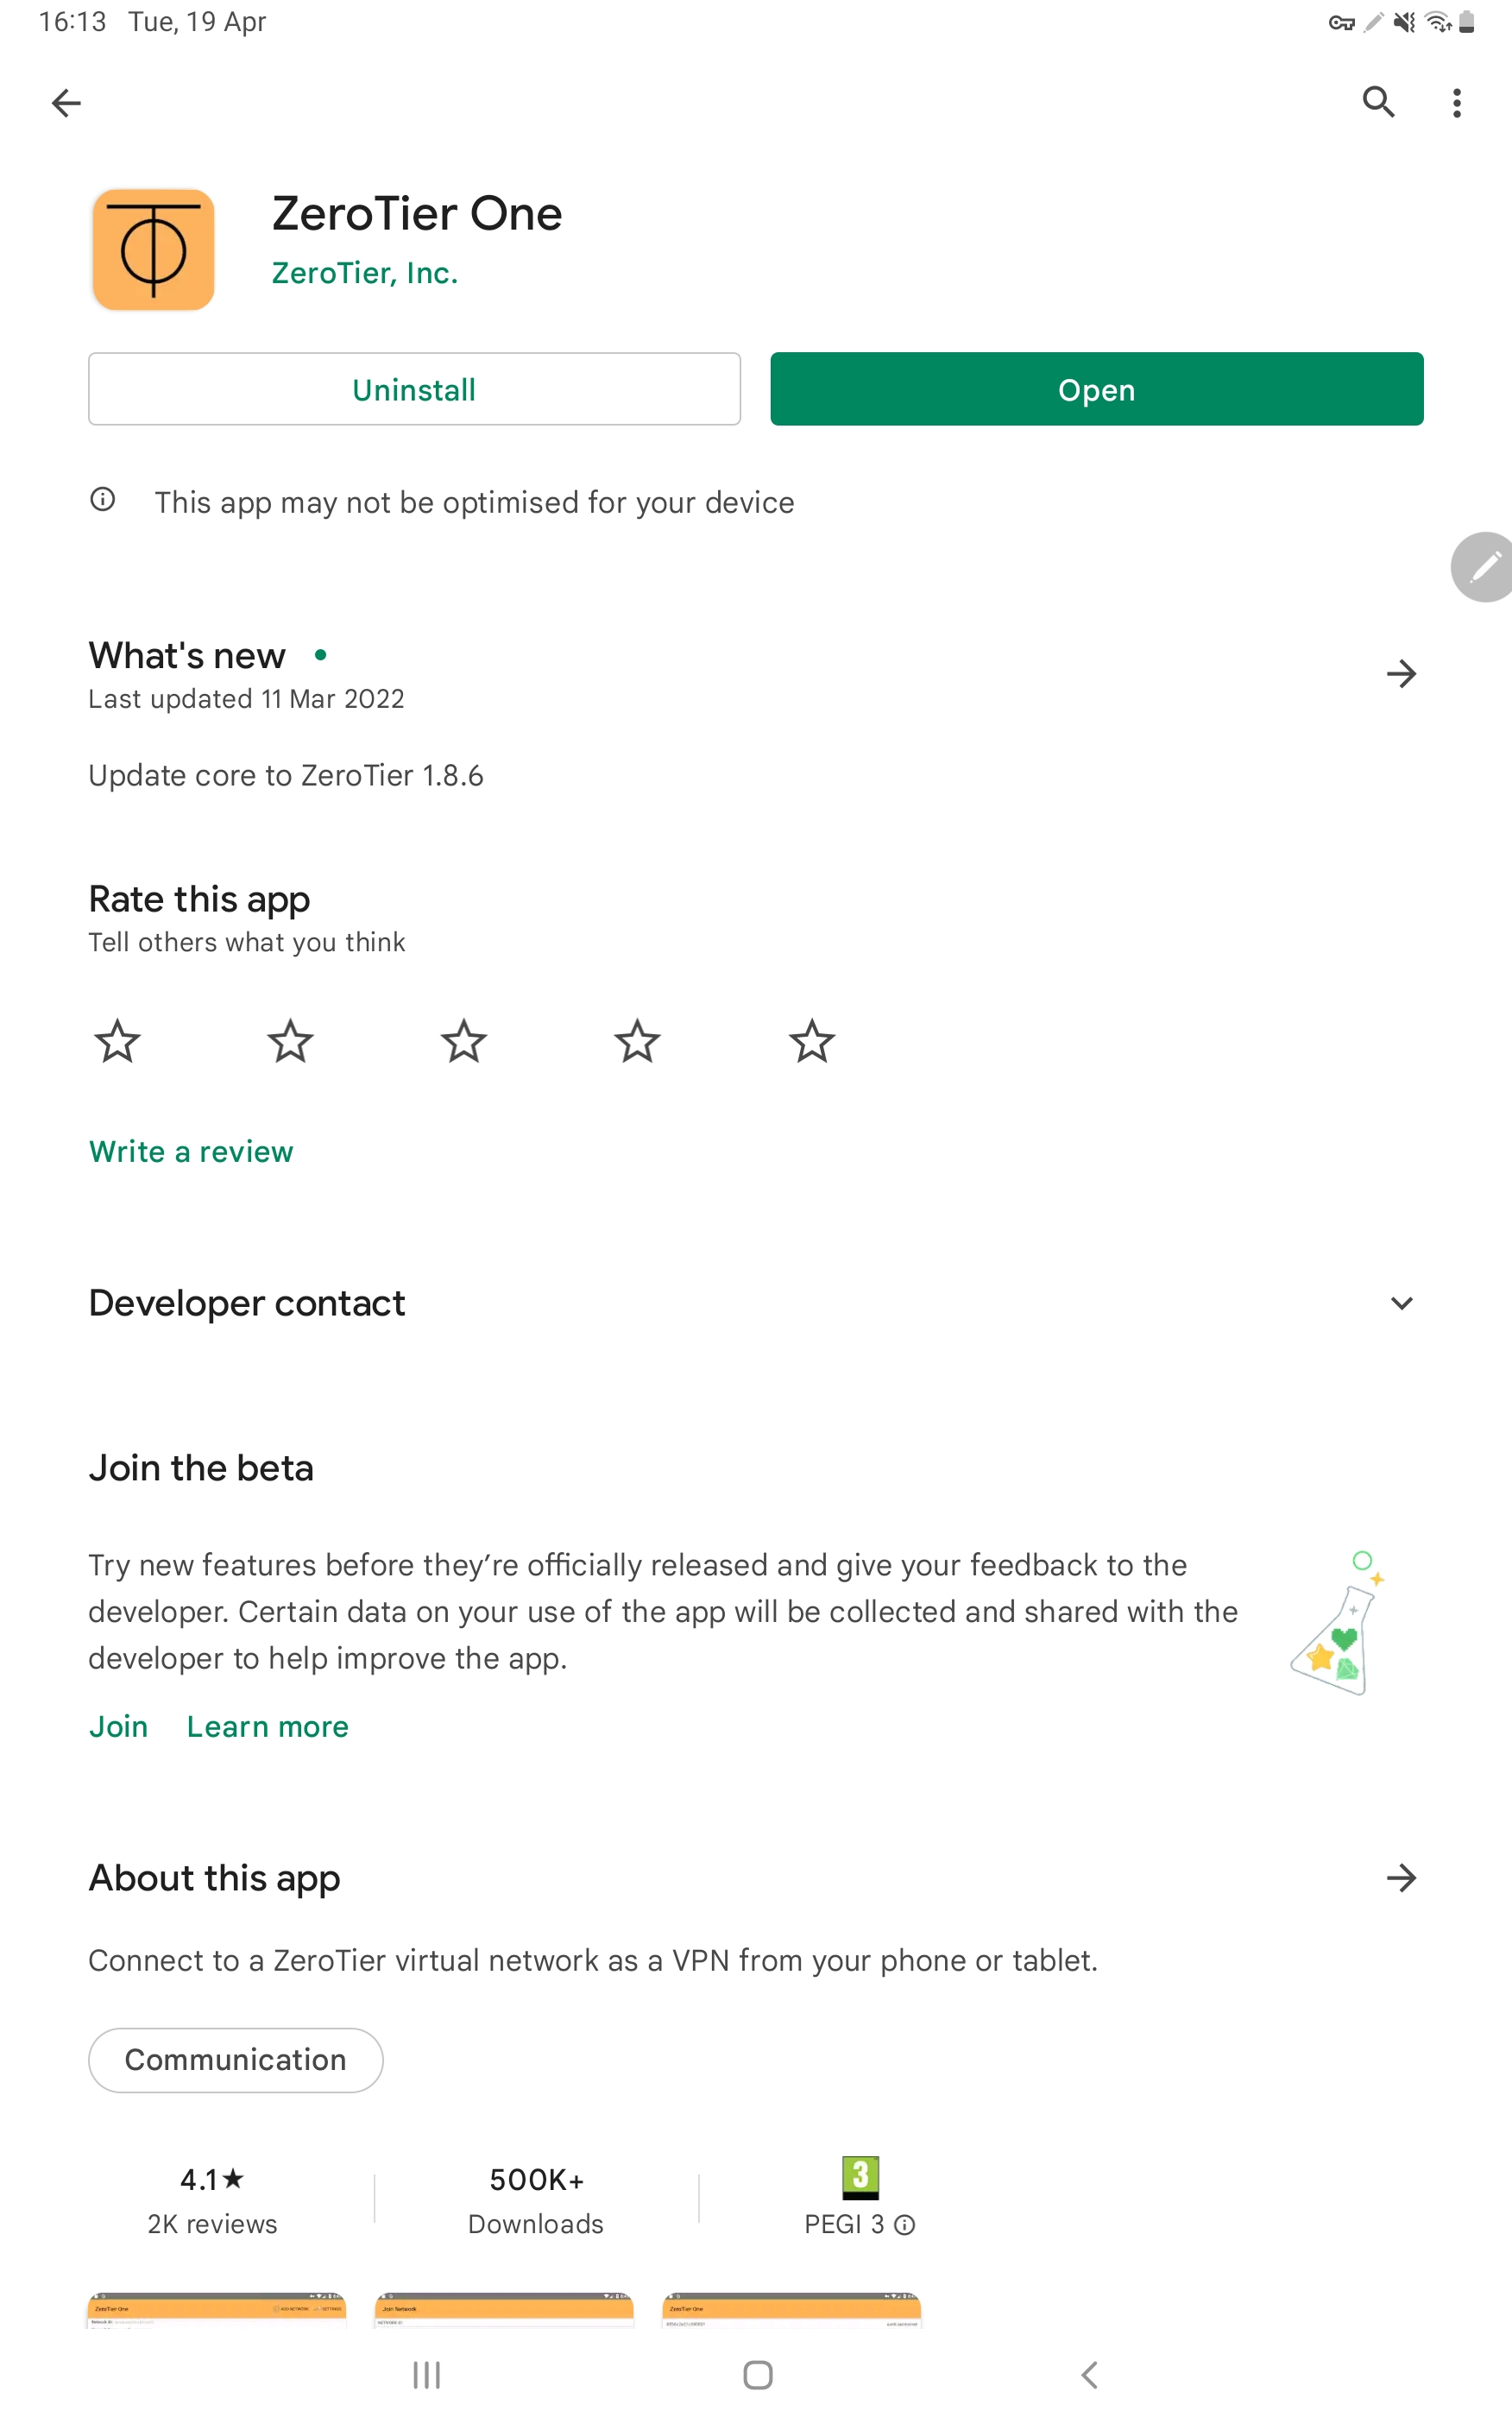
\includegraphics[scale=0.2]{1.jpg} 
\end{center}
\newpage
\section{Podłączenie do sieci}
Otwieramy aplikację Zerotier One i klikamy w ikonę " + ", aby połączyć się z nową siecią. W segmencie " NETWORK ID " podajemy interesujące nas id: " 83048a0632d2b7a6 ". Wybieramy opcję " NETWORK DNS " i klikamy przycisk " Add Network " znajdujący się na dole ekranu. Przesuwamy żółty suwak w celu połączenia z siecią.
\vspace{0.5cm}
\begin{center}
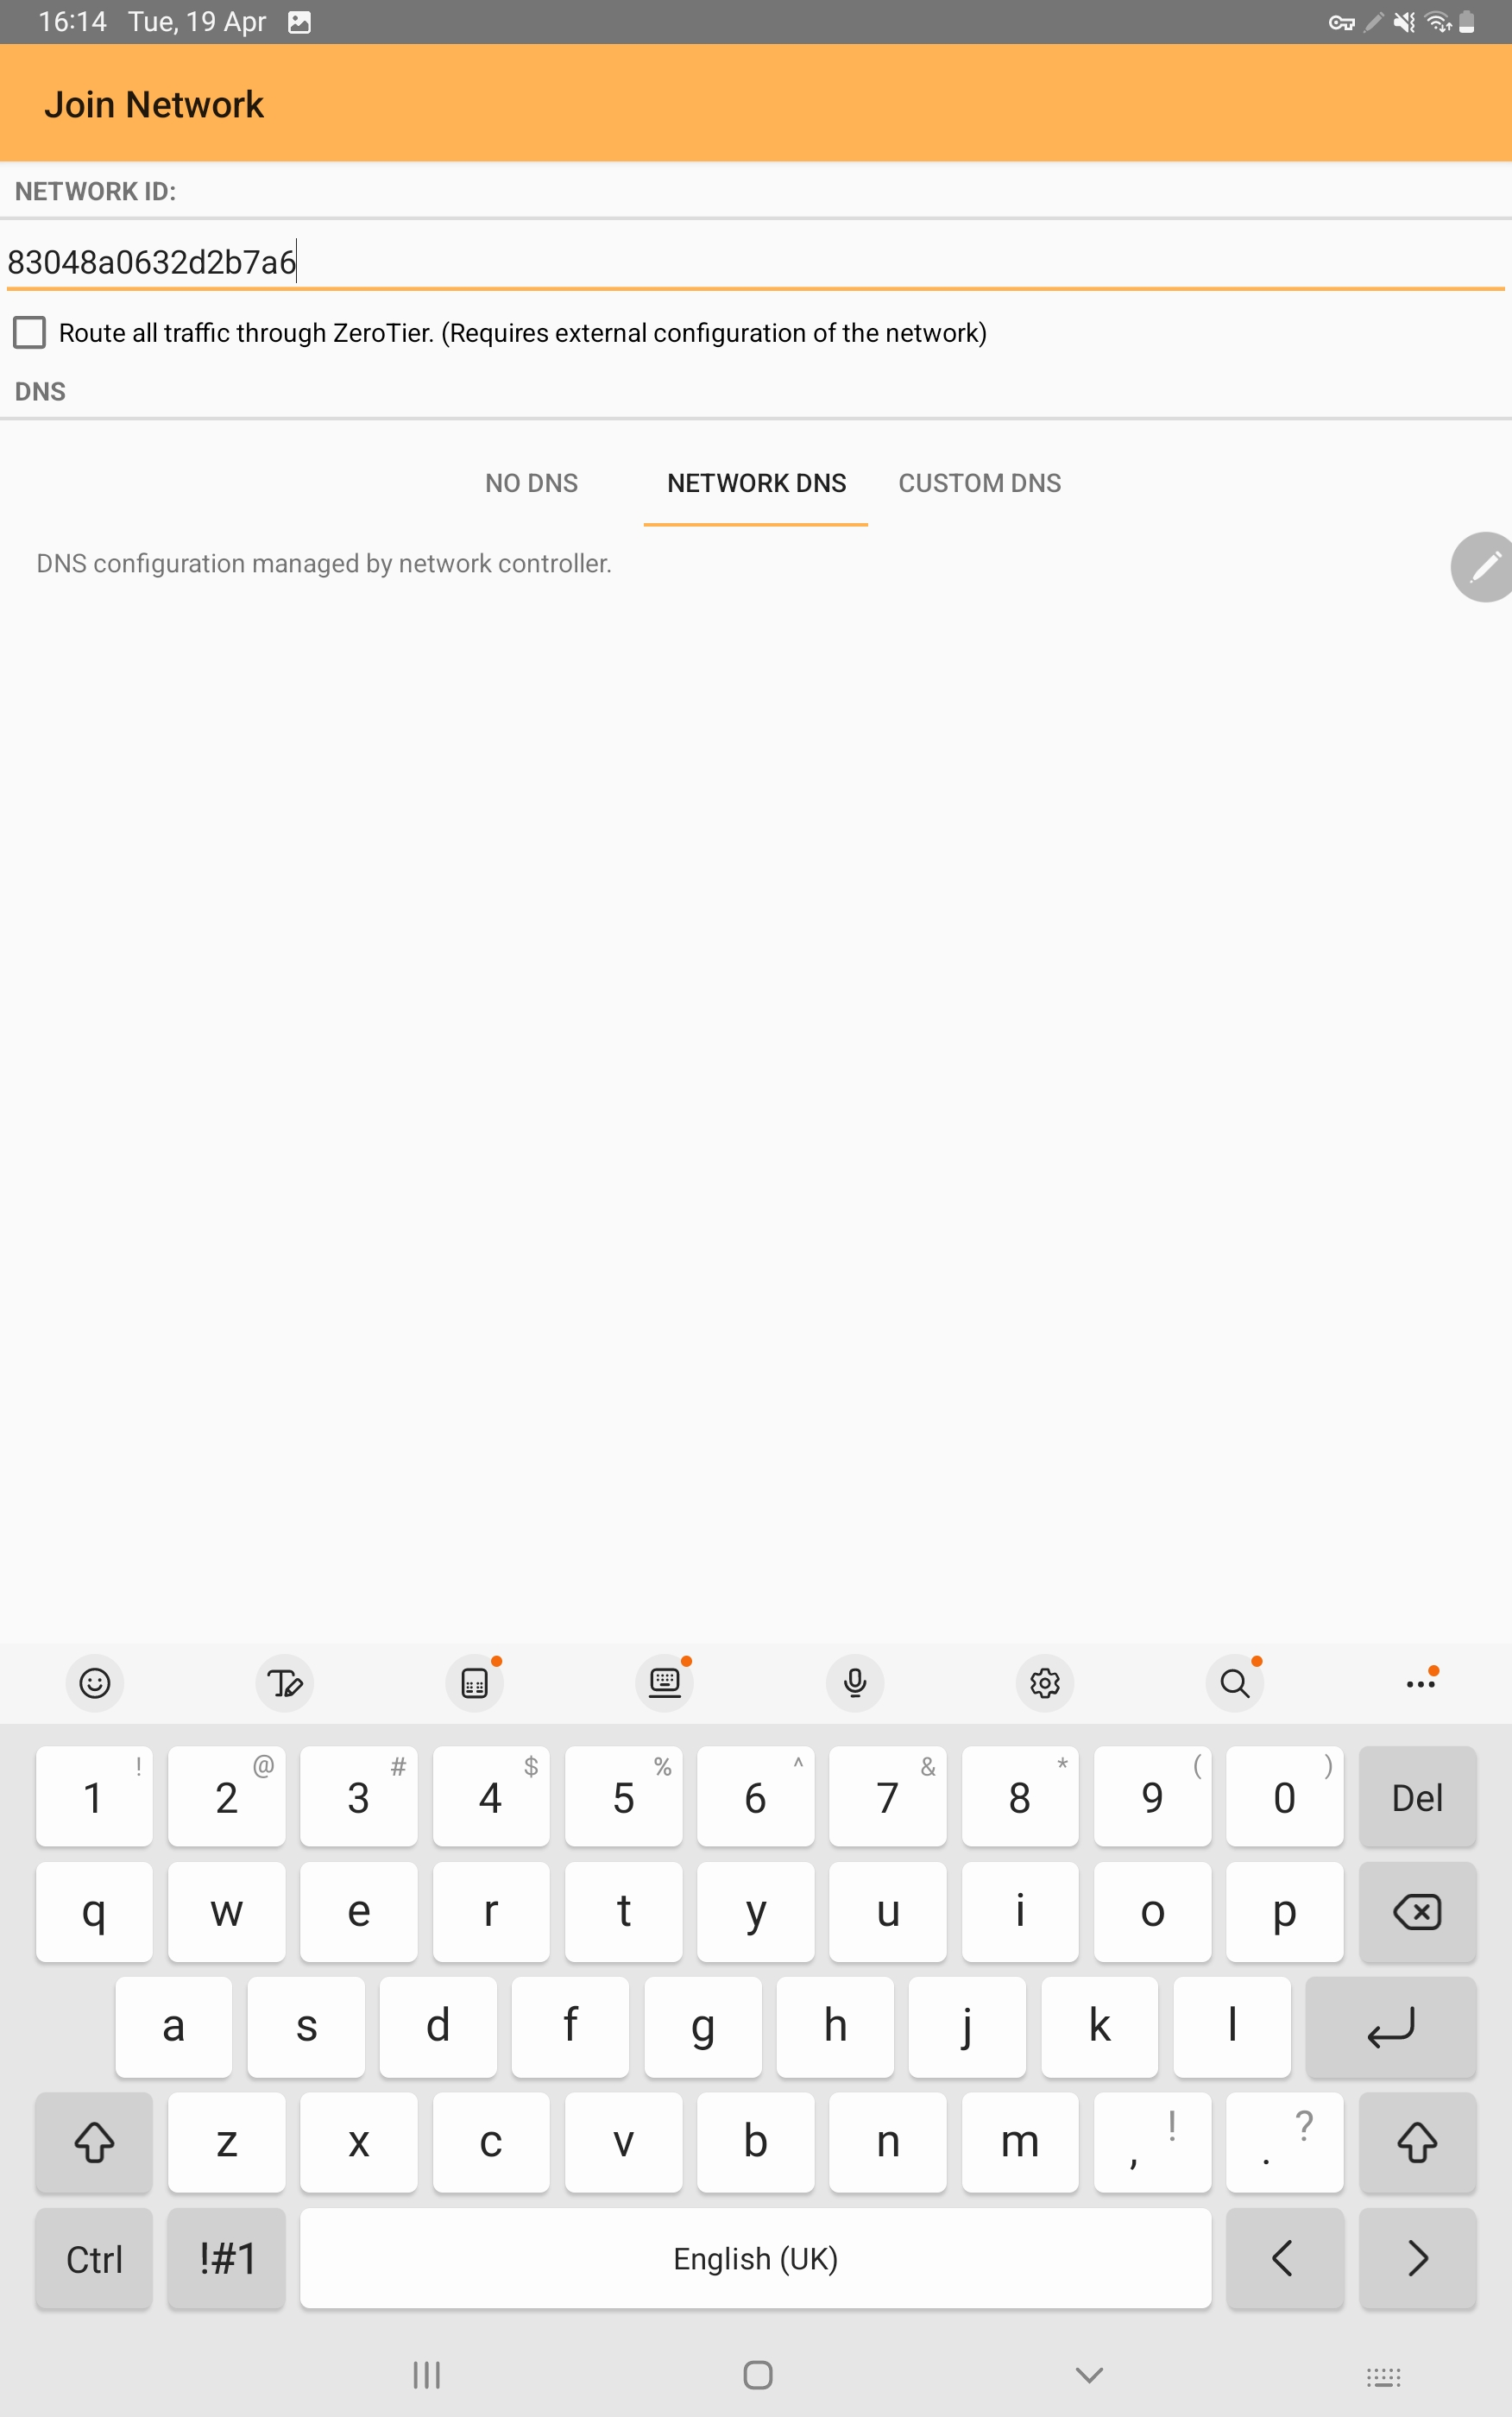
\includegraphics[scale=0.2]{2.jpg} 
\end{center}
\newpage
Aby uzyskać autoryzację połączenia musimy zgłosić się do prowadzącego laboratoria w celu dodania id naszego urządzenia ( znajduje się ono w lewej dolnej części ekranu aplikacji ZeroTier One po próbie podłączenia do sieci ) do puli urządzeń posiadających prawo dostępu do sieci.
\vspace{0.5cm}
\begin{center}
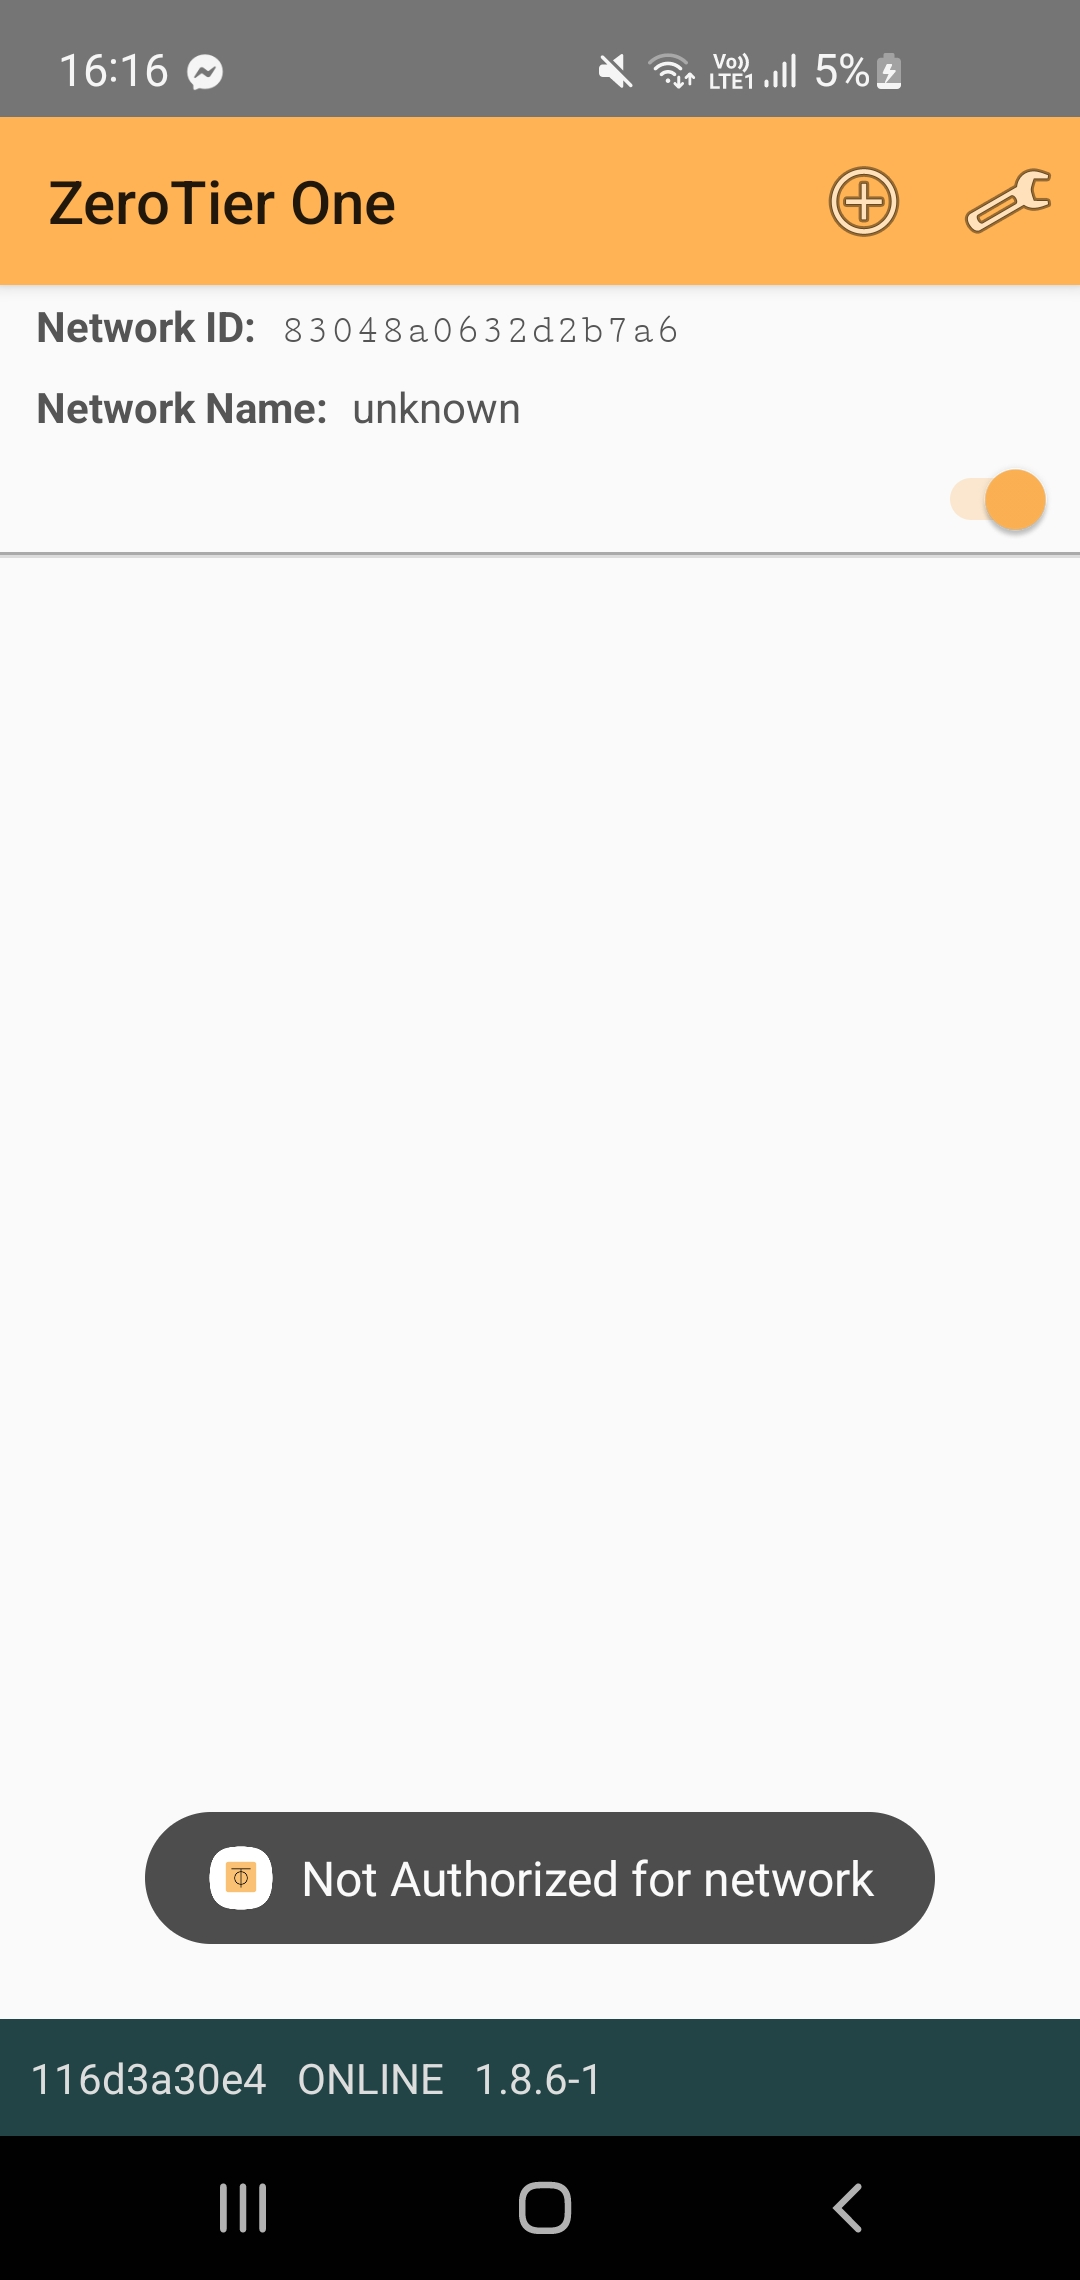
\includegraphics[scale=0.25]{3.jpg} 
\end{center}
\newpage
\section{Uzyskanie dostępu do zasobów dyskowych bezpośrednio z urządzenia}
Przechodzimy do menedżera plików do sekcji " Network storage ".
\vspace{0.5cm}
\begin{center}
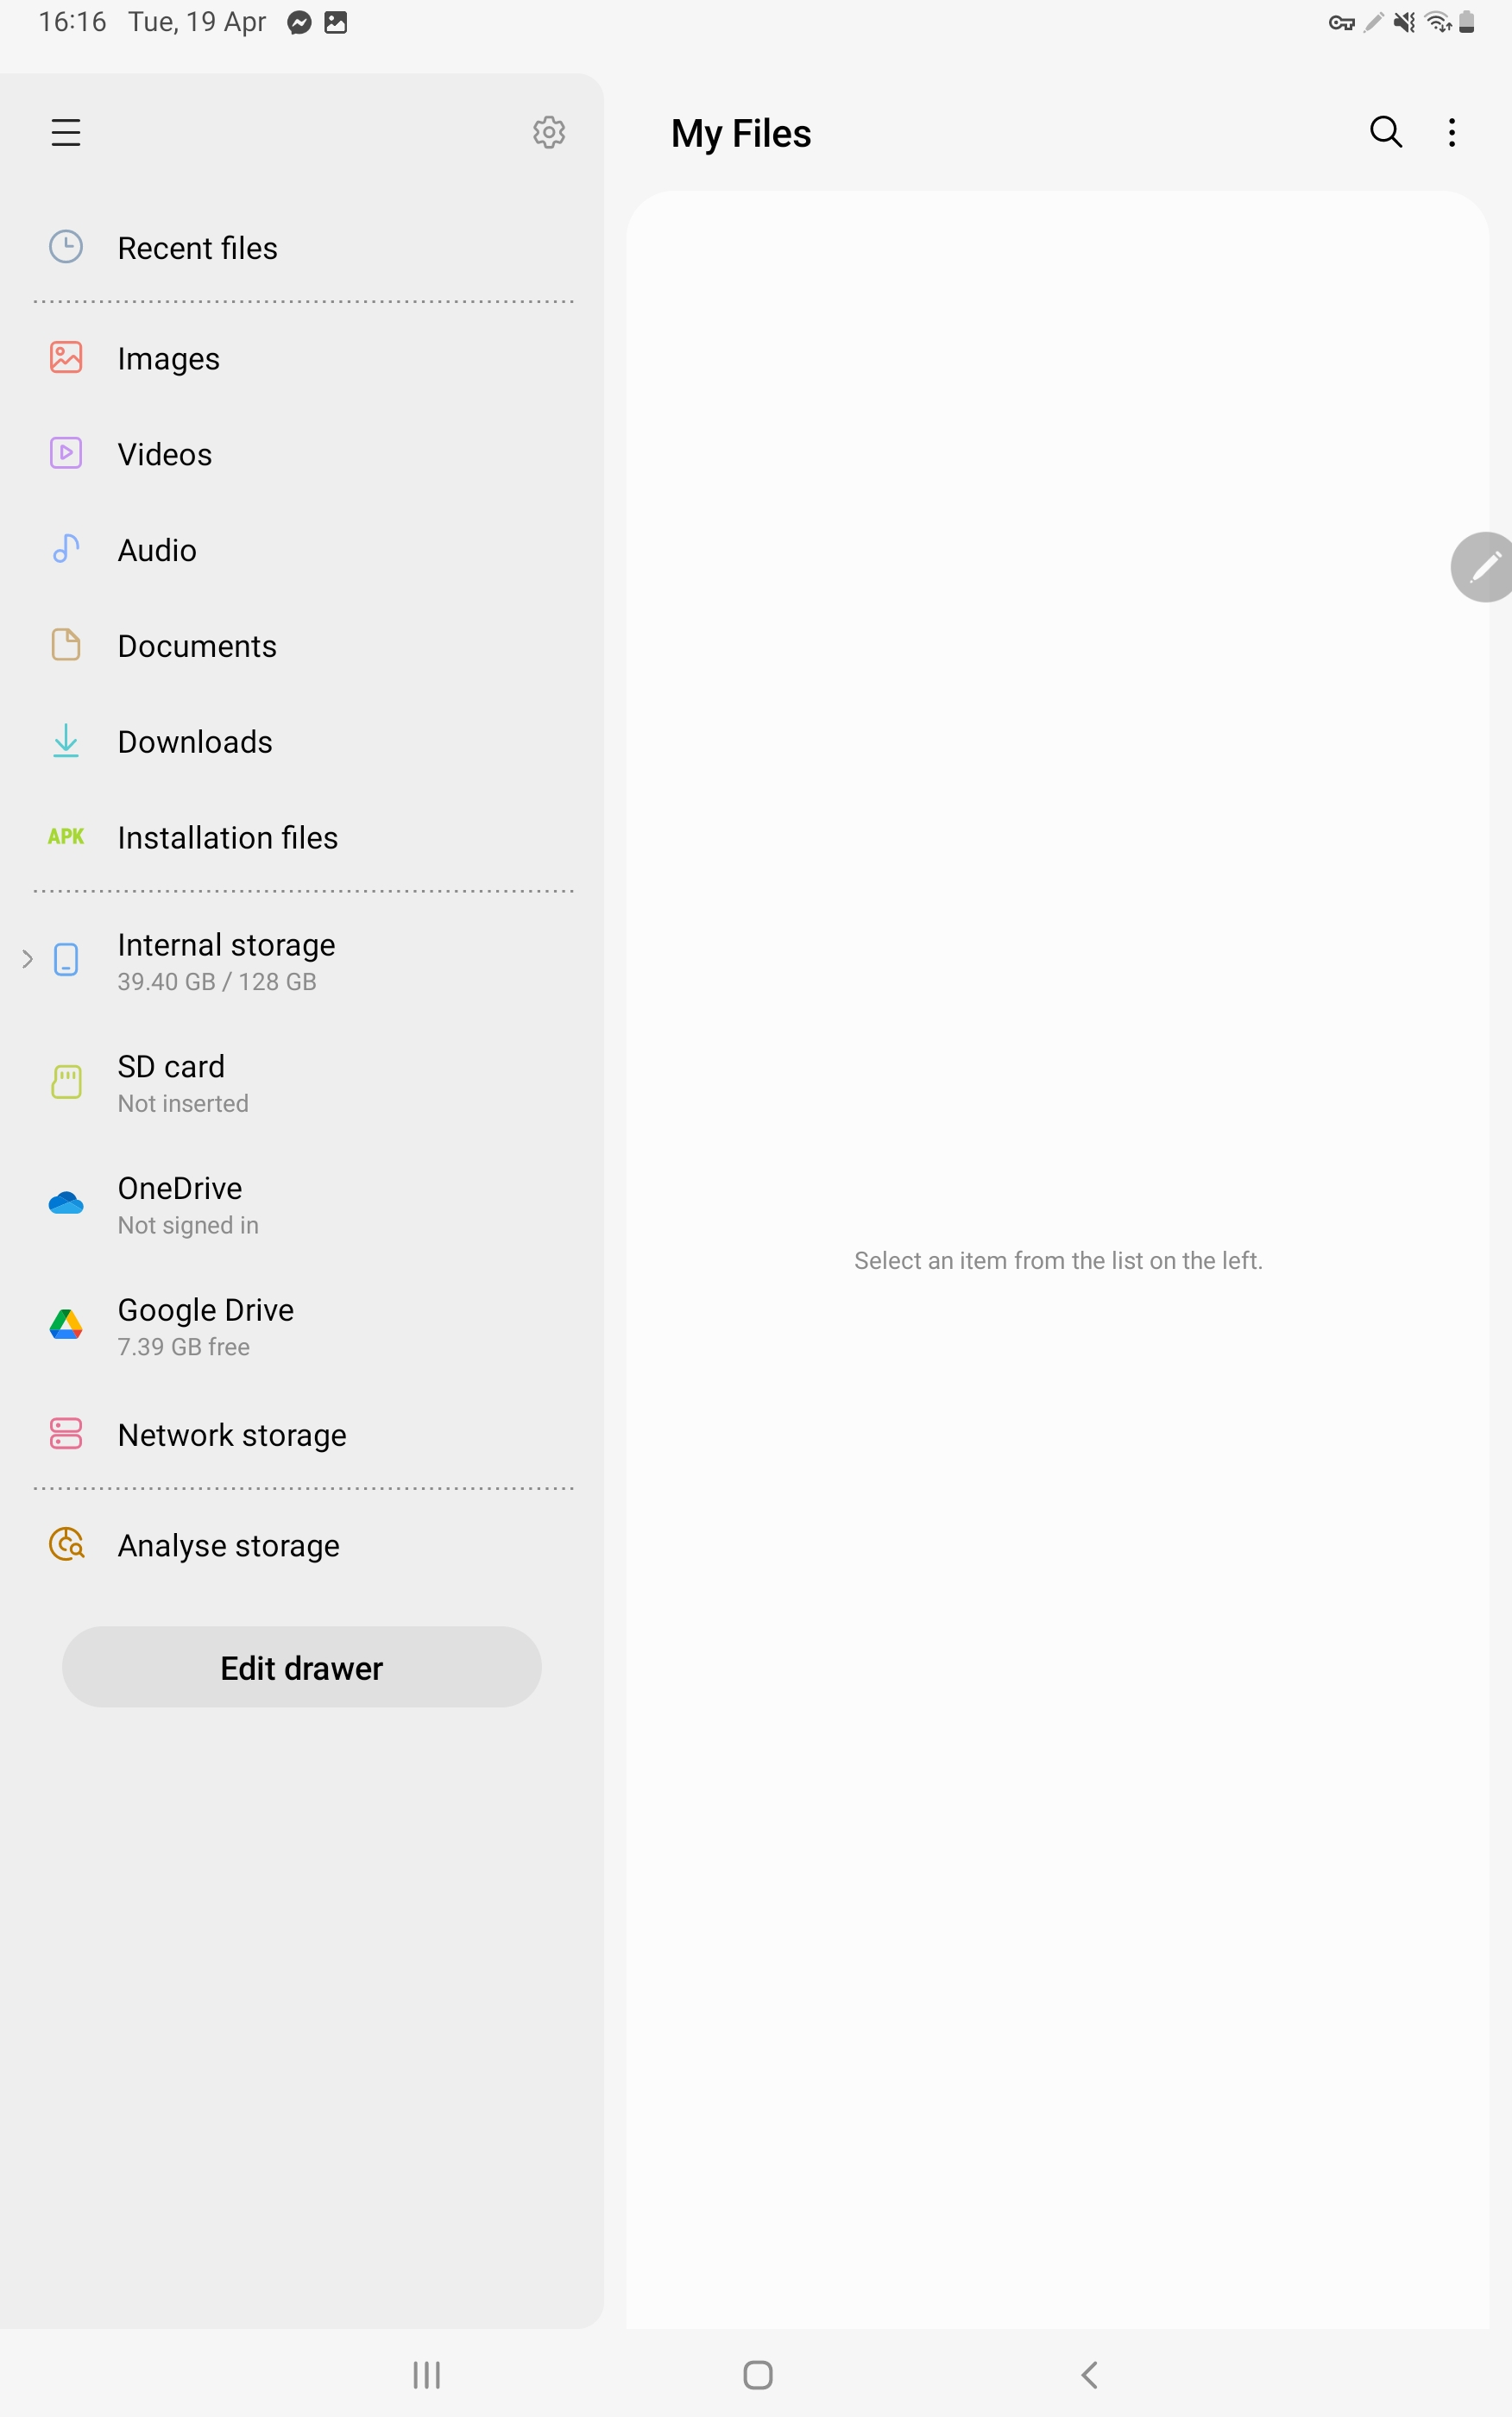
\includegraphics[scale=0.2]{4.jpg} 
\end{center}
\newpage
Klikamy w ikonę " + " znajdującą się w prawej górnej części ekranu i wybieramy opcję " Network drive (SMB) ".
\vspace{0.5cm}
\begin{center}
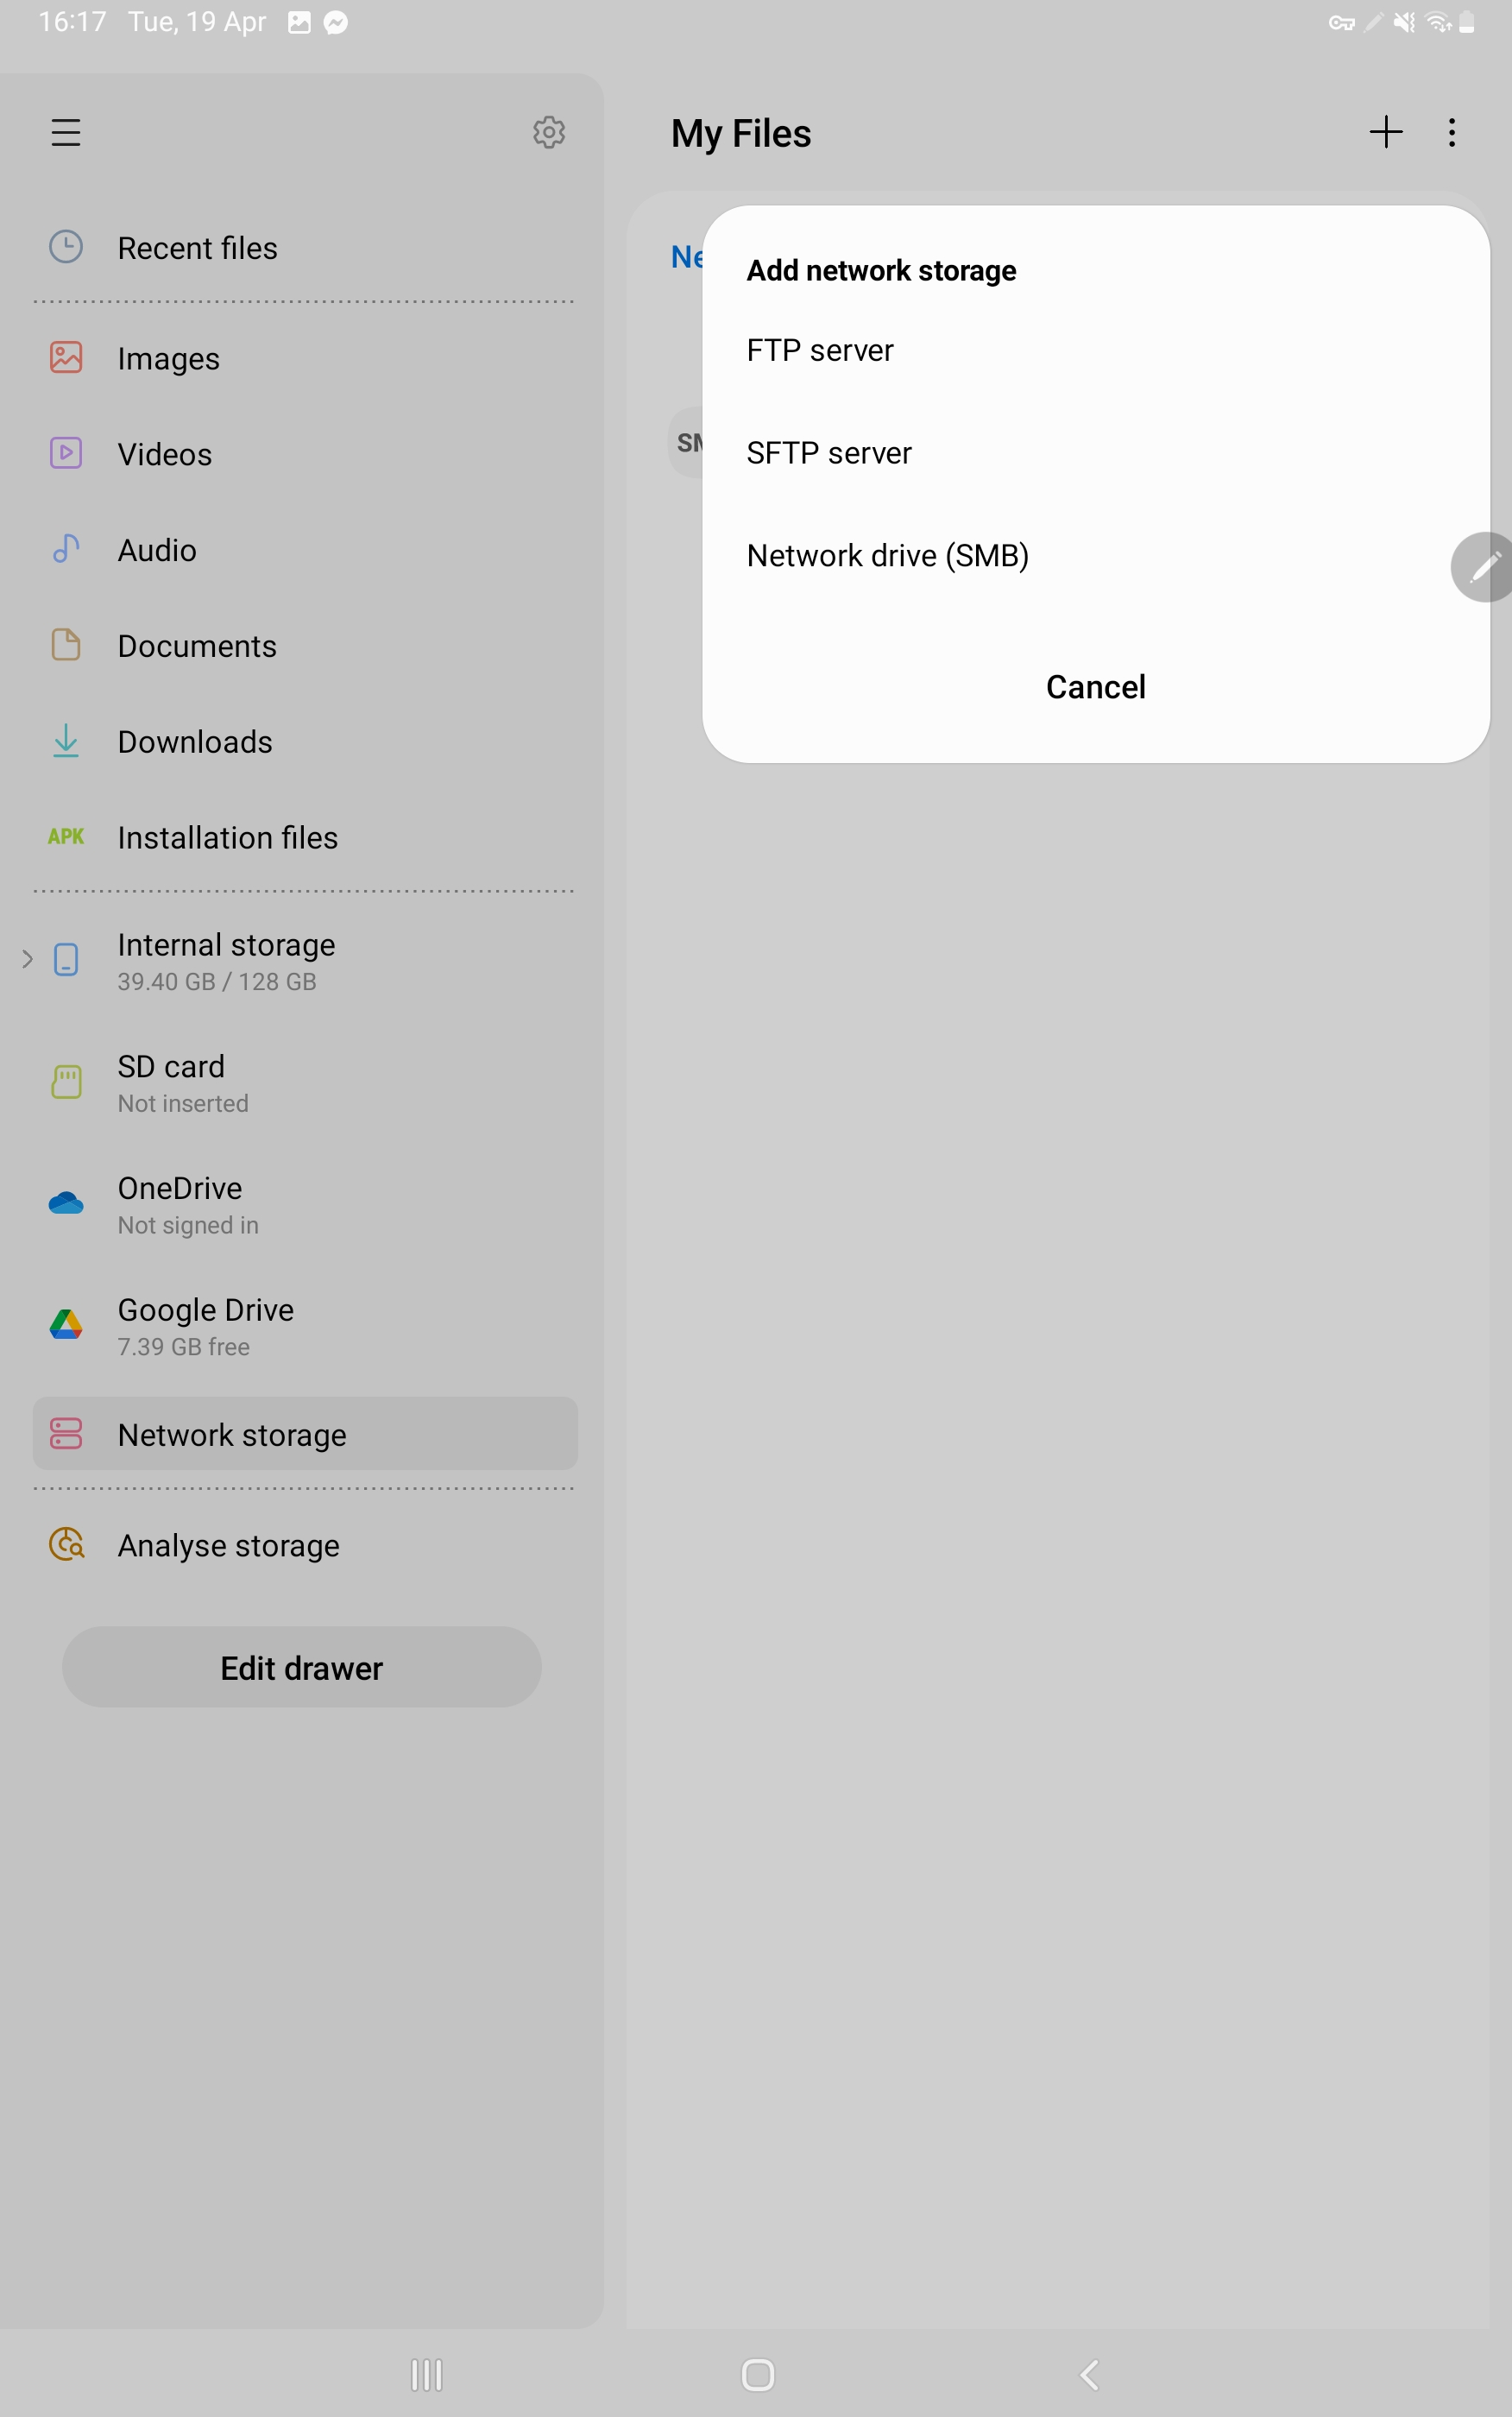
\includegraphics[scale=0.2]{5.jpg} 
\end{center}
\newpage
Wybieramy opcję ręcznego dodania dysku sieciowego.
\vspace{0.5cm}
\begin{center}
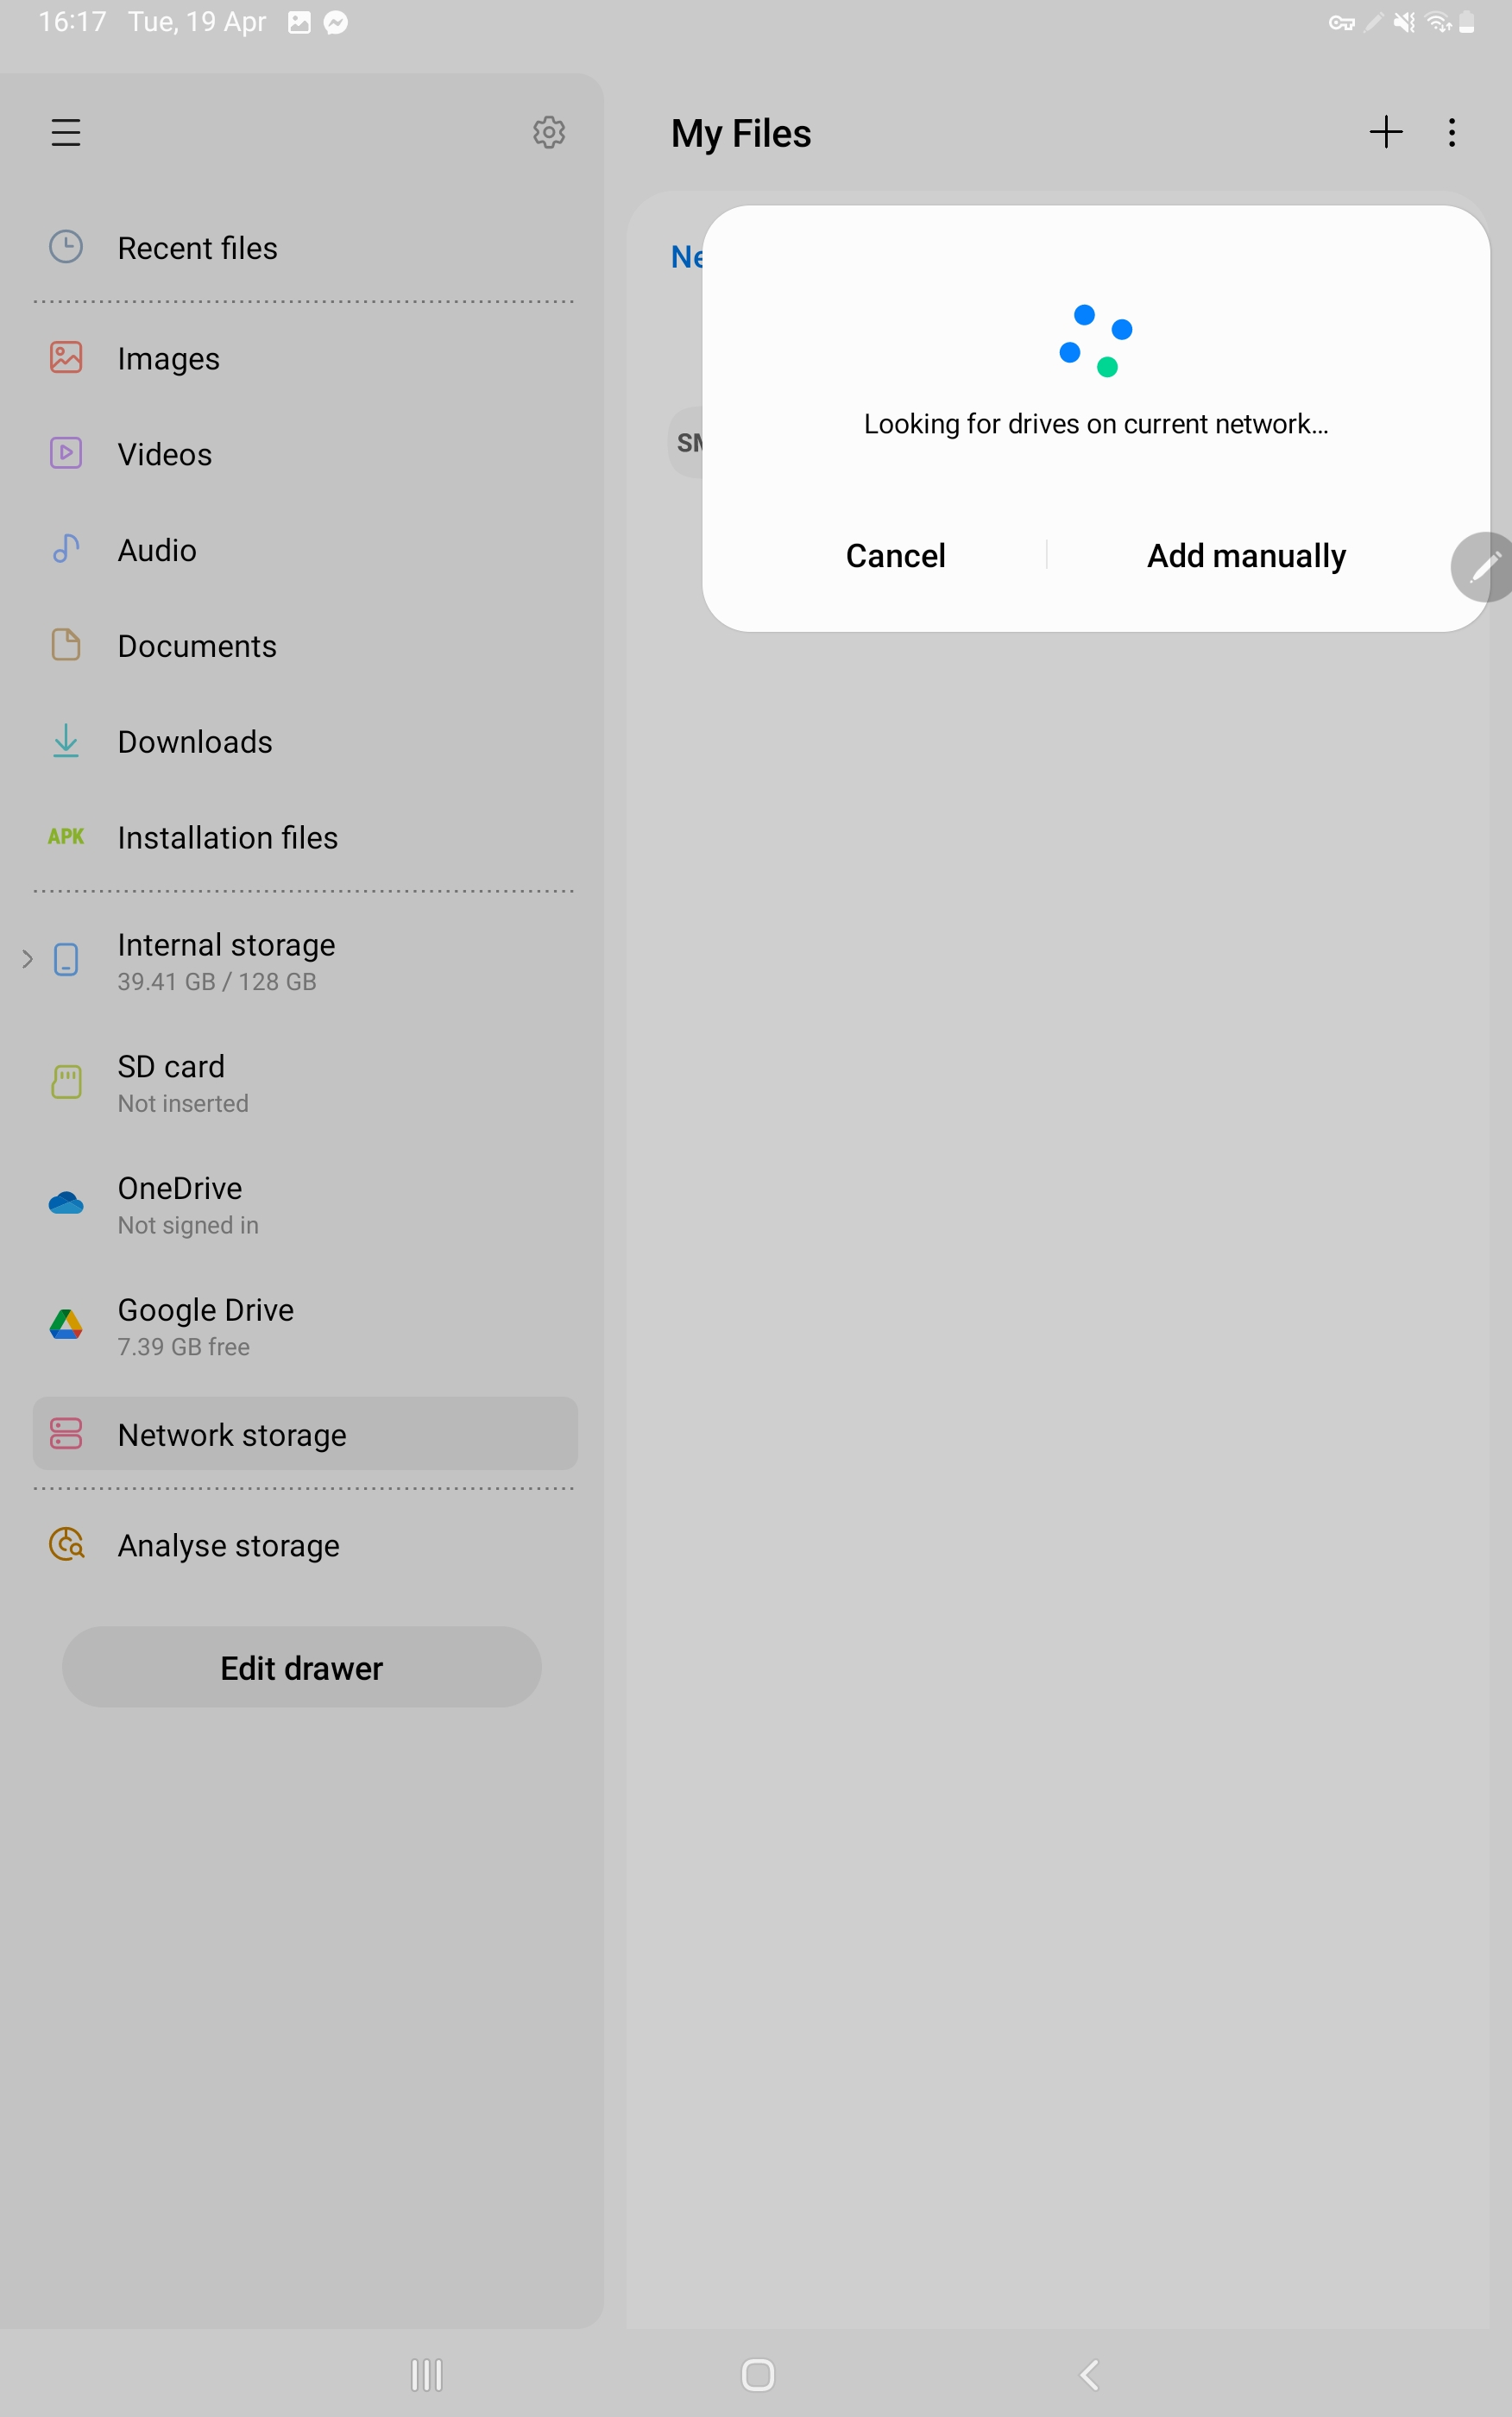
\includegraphics[scale=0.2]{6.jpg} 
\end{center}
\newpage
Następnie dodajemy dysk sieciowy wpisując następujące dane logowania:
\vspace{0.5cm}
\begin{center}
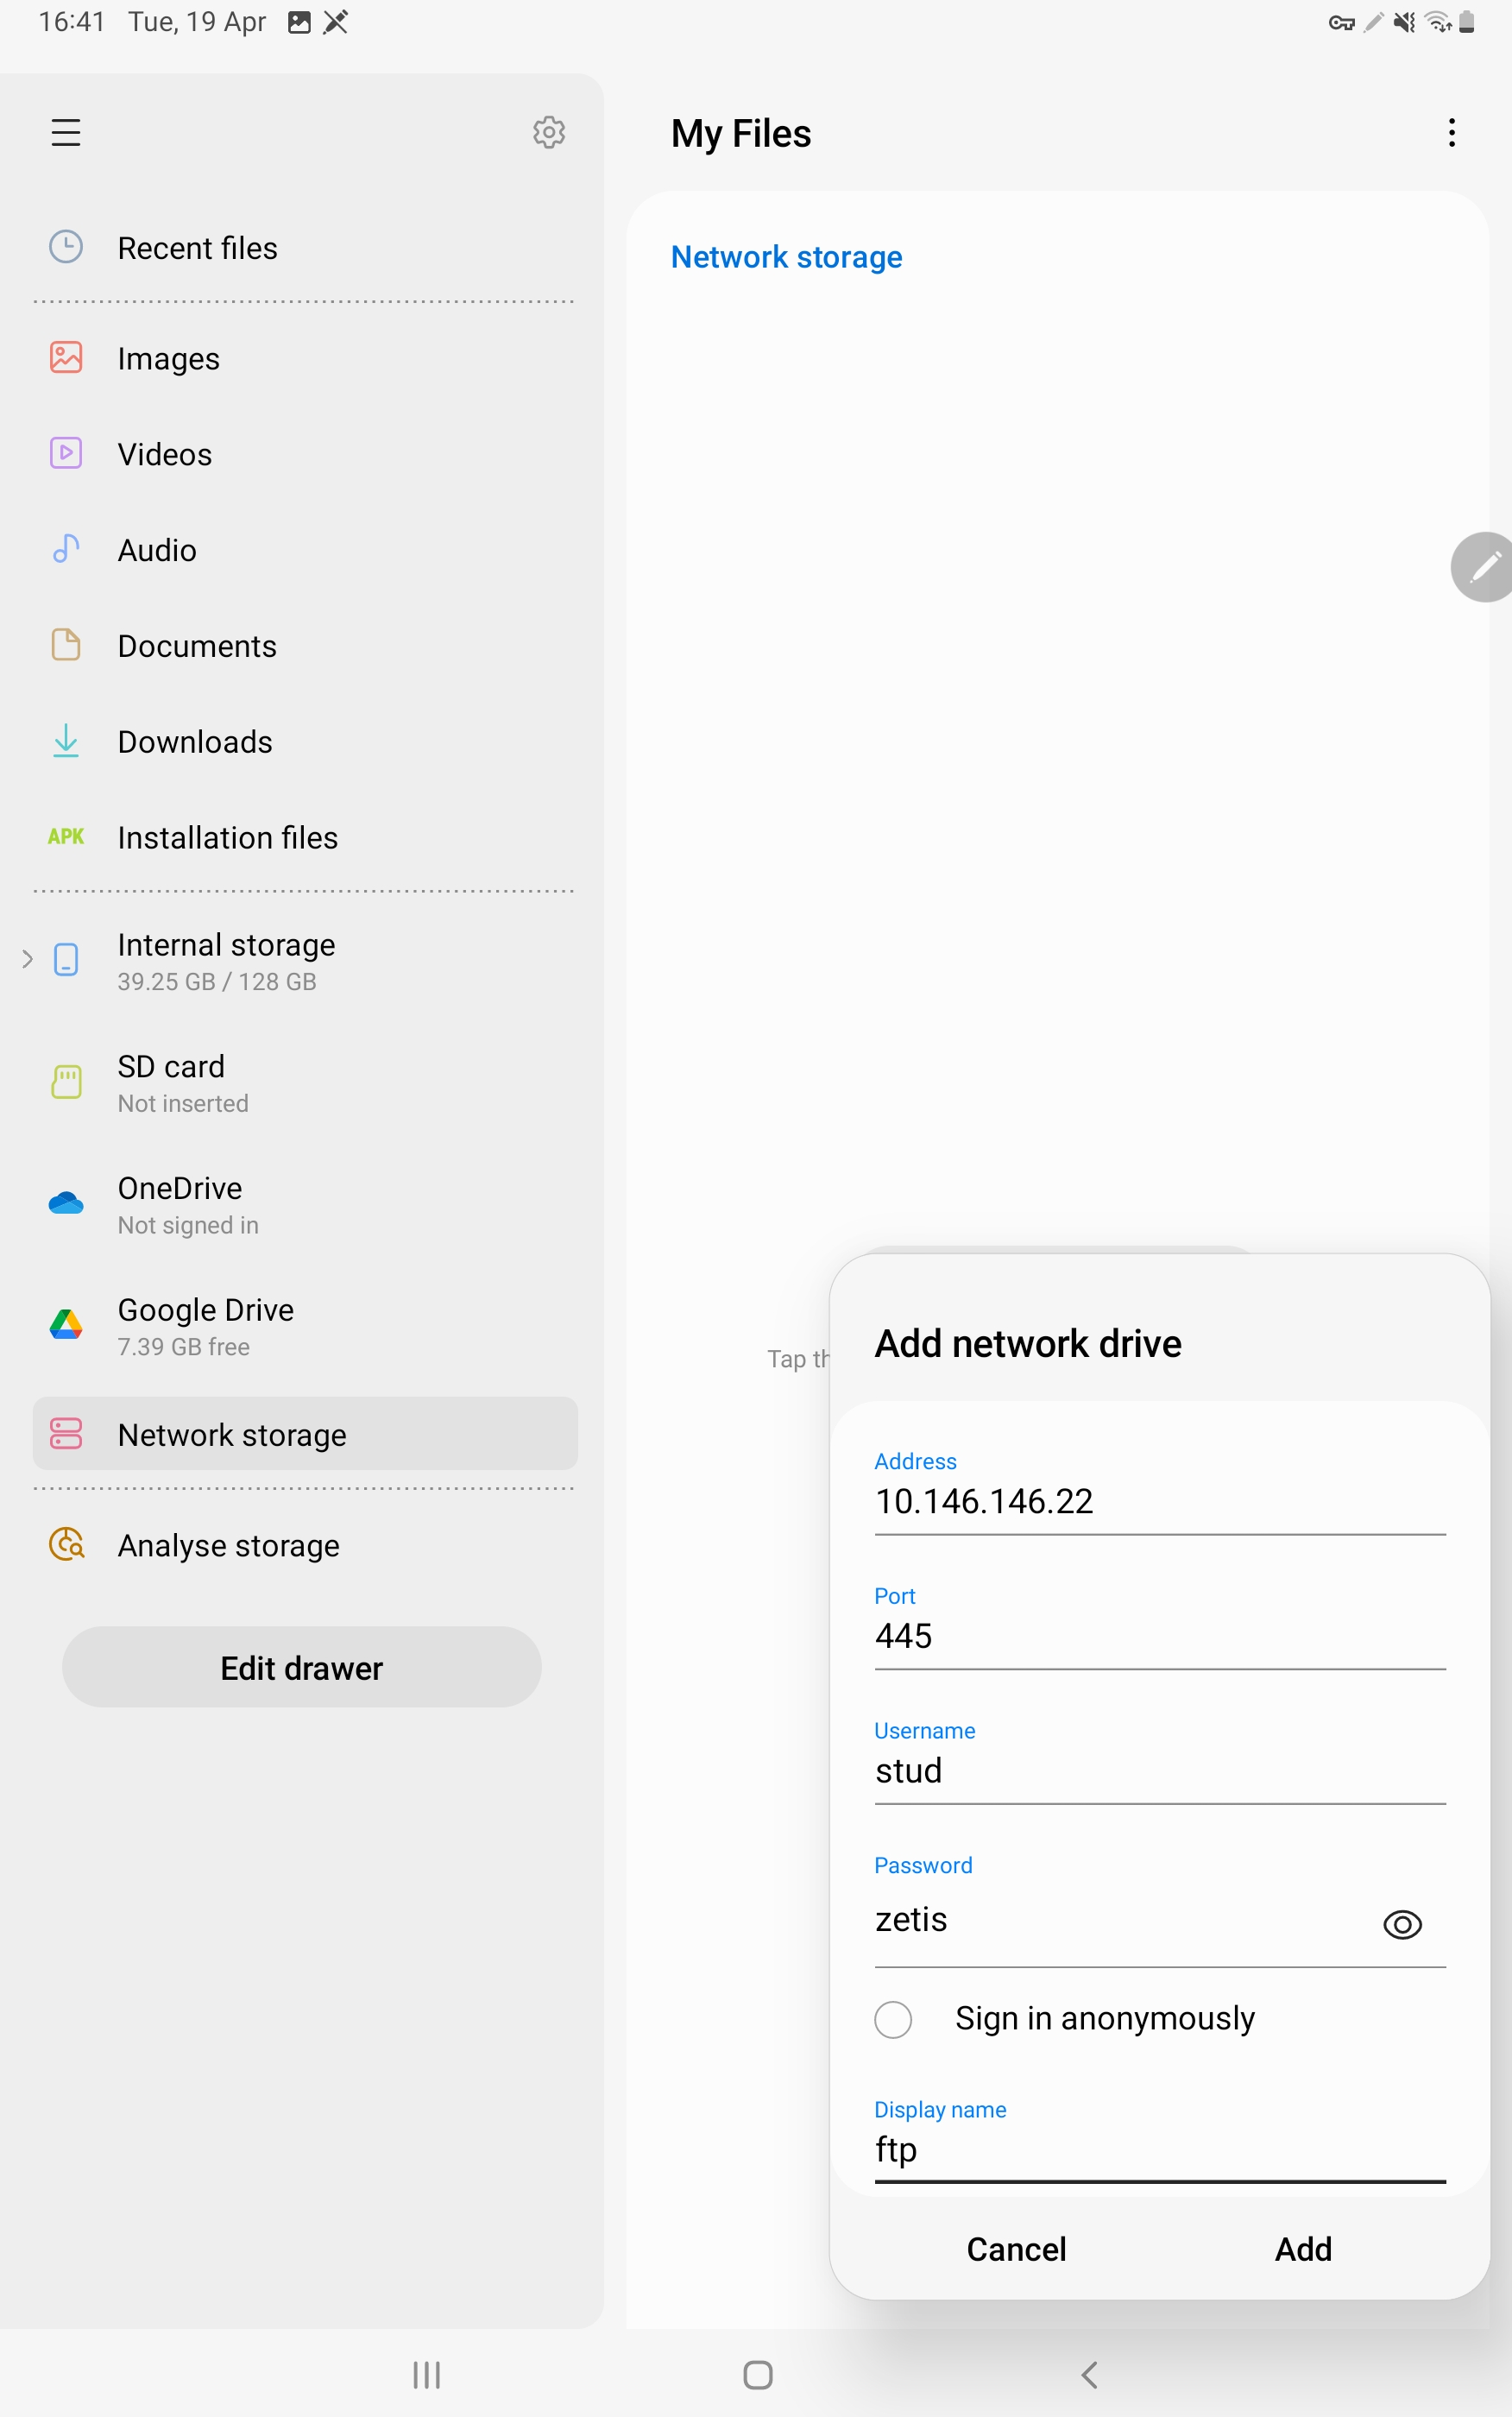
\includegraphics[scale=0.2]{7.jpg} 
\end{center}
\newpage
Po wykonaniu pełnej sekwencji poleceń powinniśmy posiadać widoczny dysk sieciowy ftp oraz móc przegladać jego zasoby.
\vspace{0.5cm}
\begin{center}
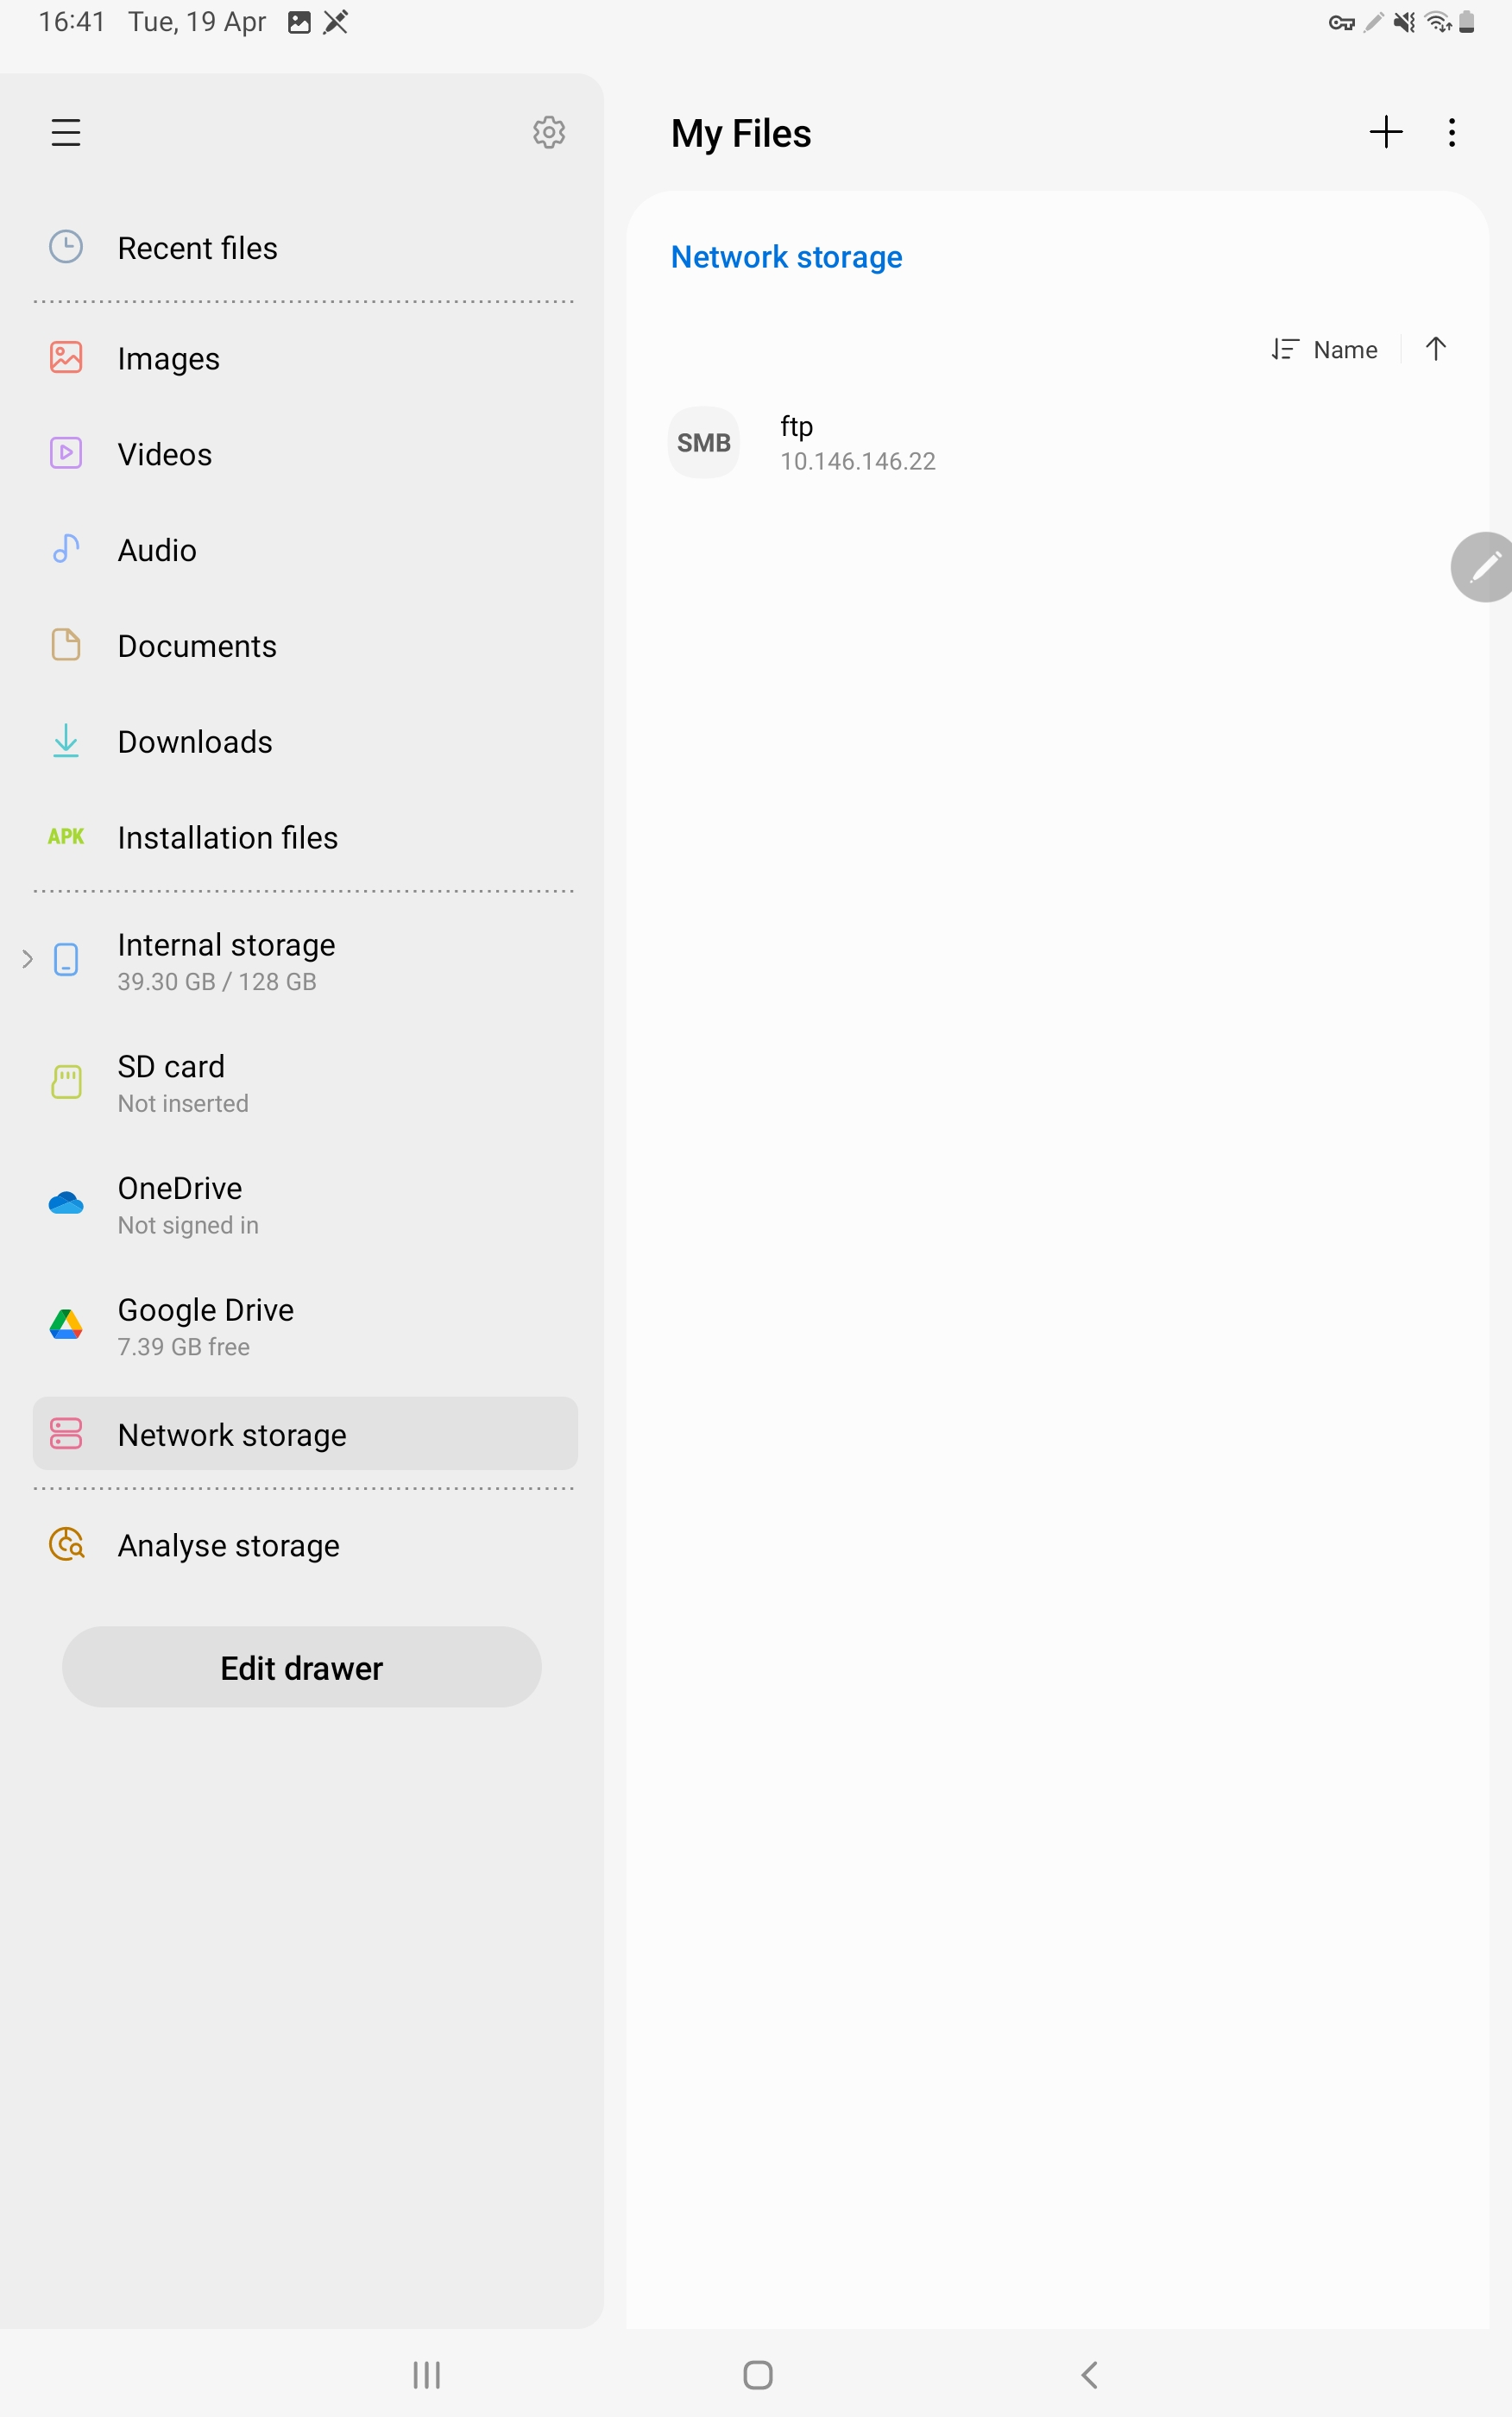
\includegraphics[scale=0.2]{8.jpg} 
\end{center}
\newpage
\begin{center}
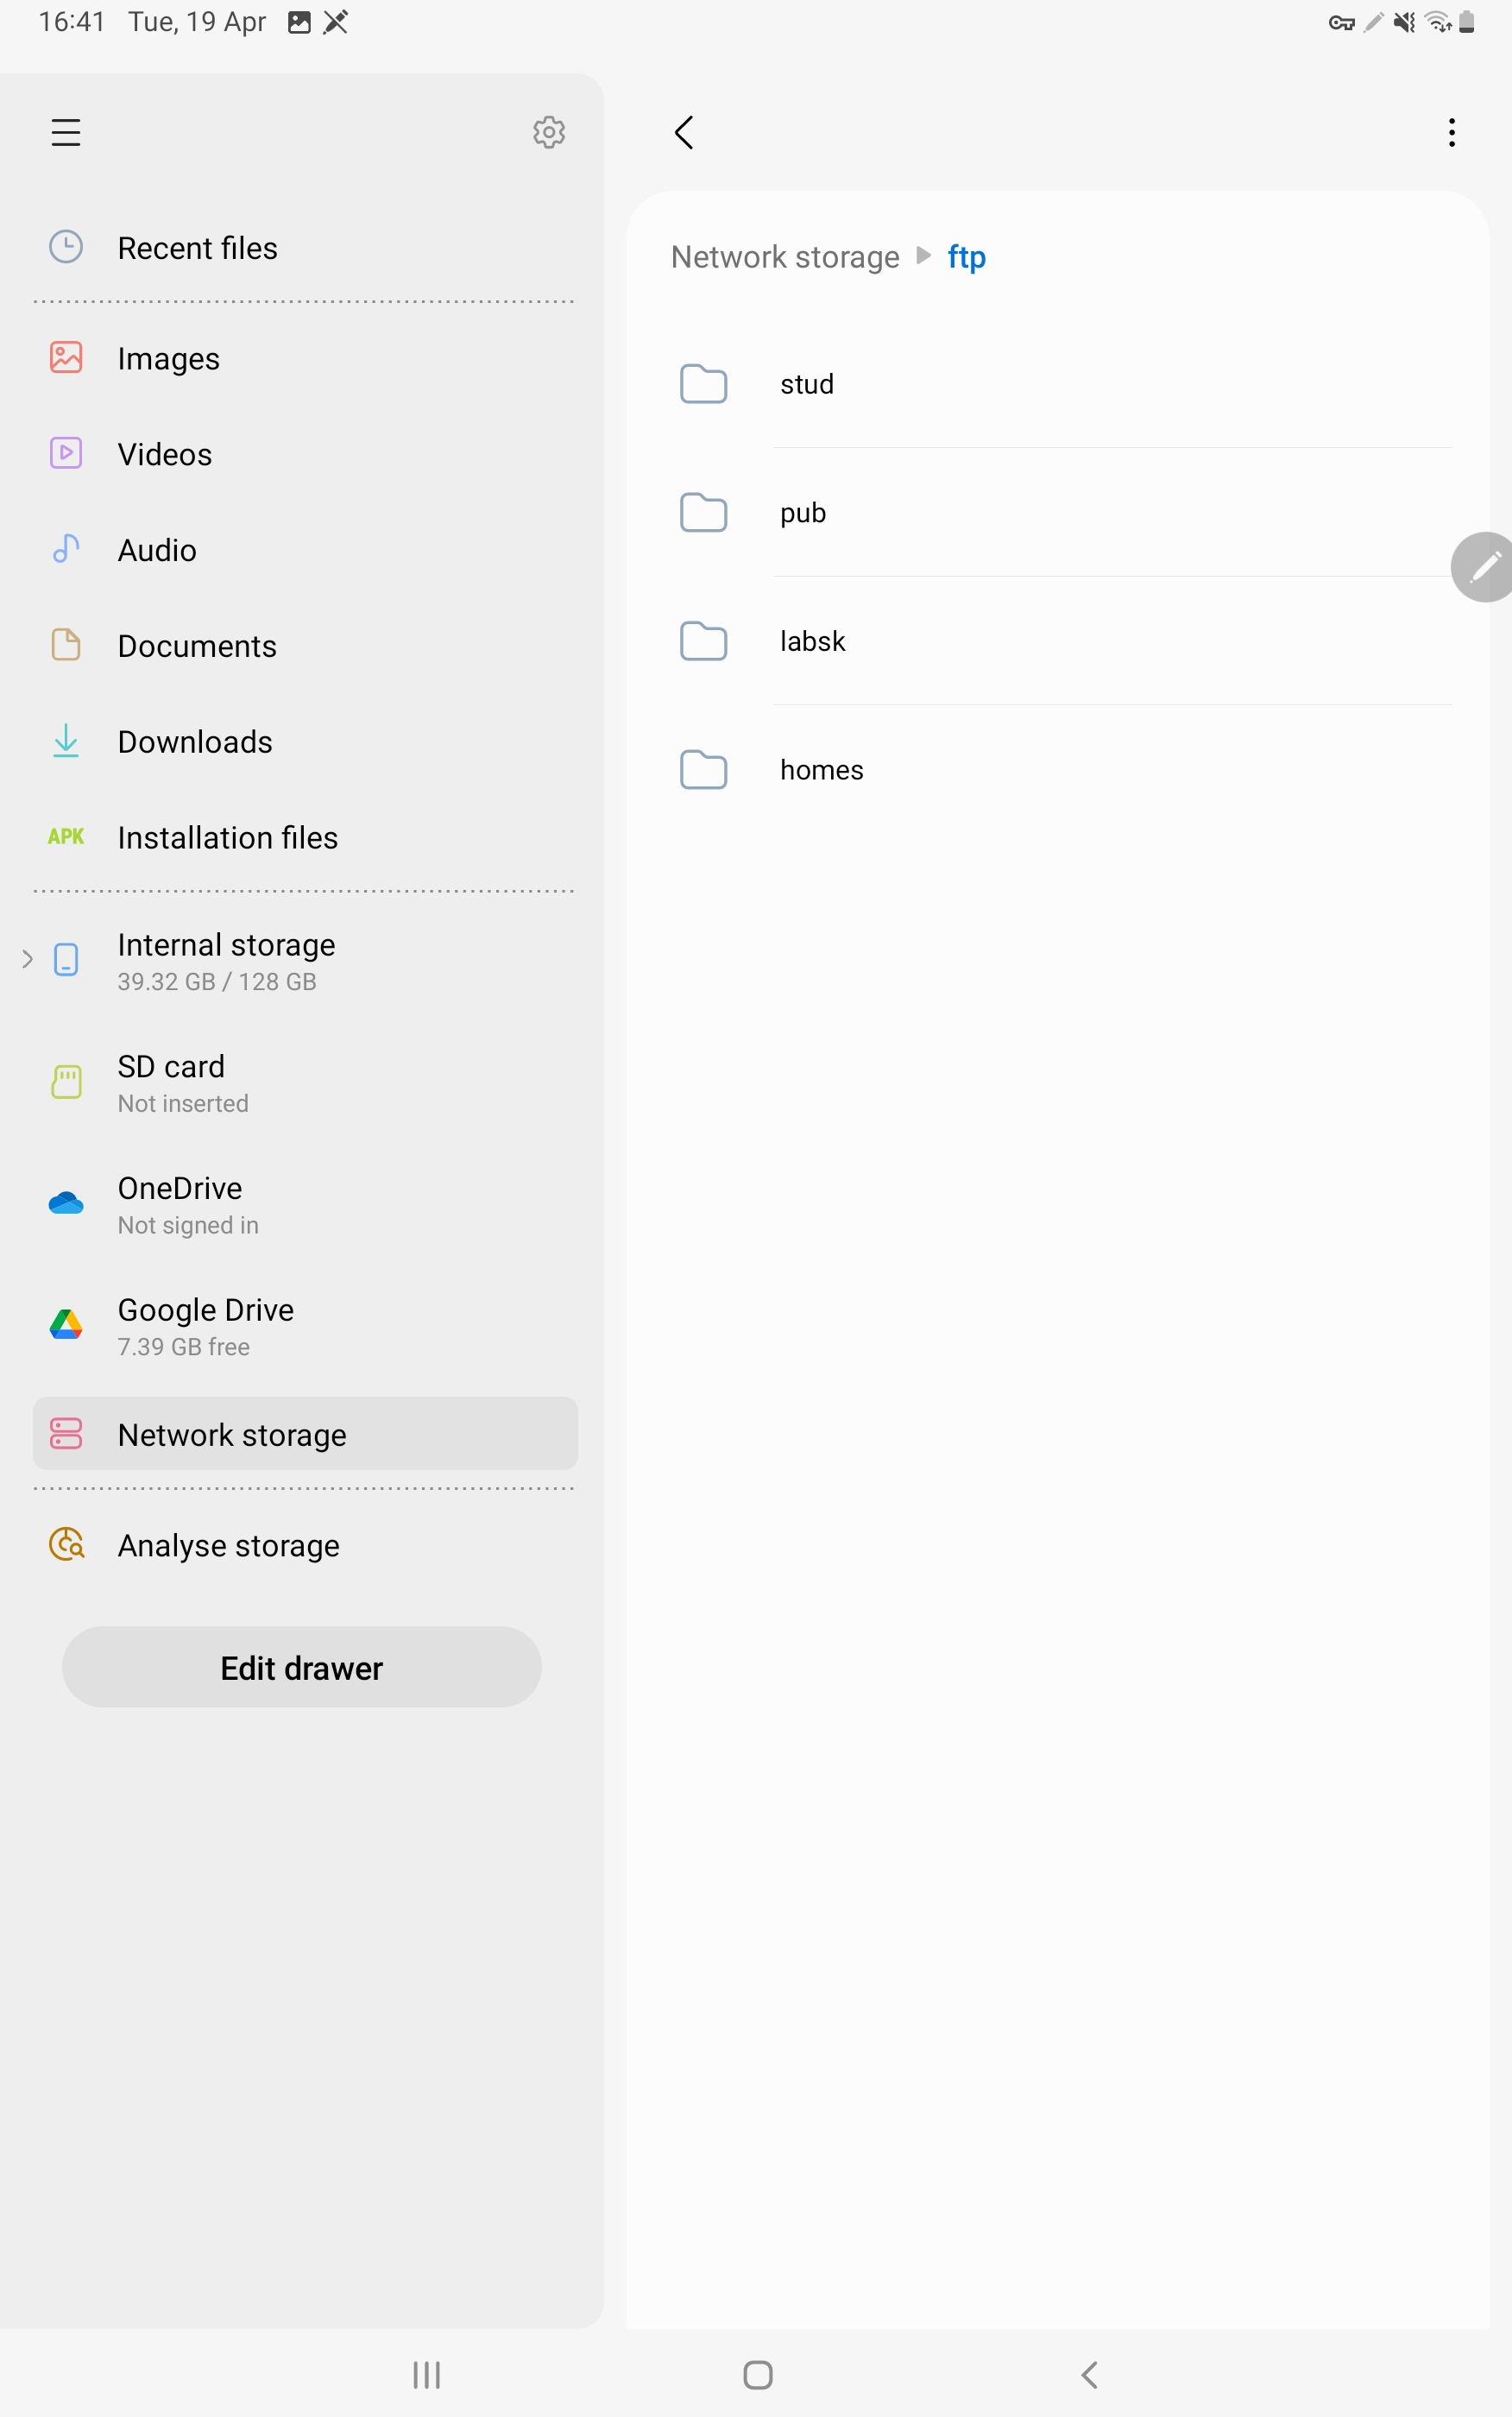
\includegraphics[scale=0.2]{9.jpg} 
\end{center}
\newpage
\end{document}

